\textbf{Oscillator System:}(\ref{fig:osc_and_match}) The Spectre simulation of the oscillator system gives (\ref{fig:osc_trans}) as it's transient waveform on \(R_L\) with frequencies shown in Figure (\ref{fig:osc_spec}). 

A maximum attainable efficiency of \(19.8\%\)(based on \(V_{cc}, V_{ee}\)) was measured.
\begin{comment}
\begin{figure}[htbp]
    \centering
    \begin{subfigure}[b]{0.49\textwidth}
        \centering
        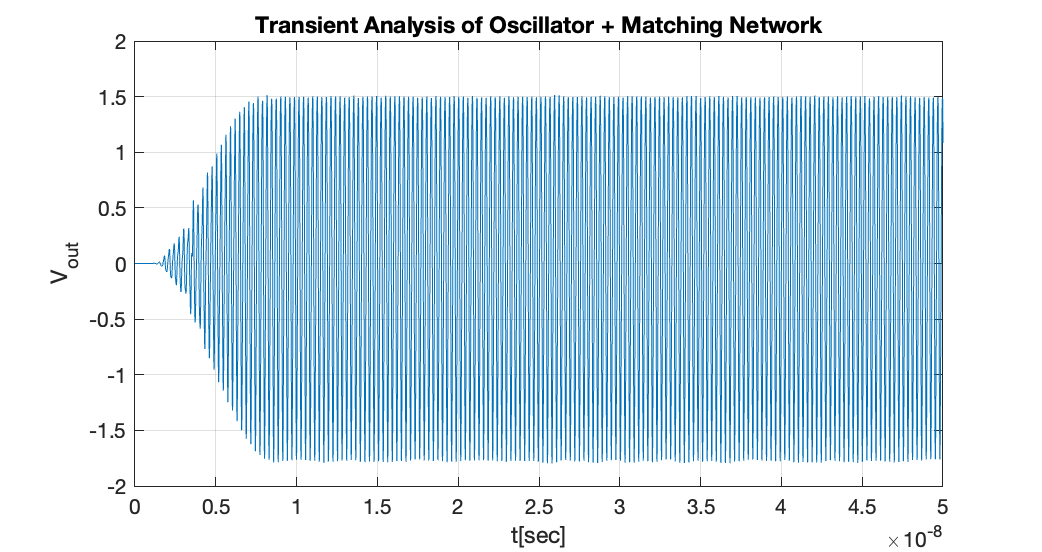
\includegraphics[width=\textwidth]{images/osc/VCO_trans.png}
        \caption{Transient Analysis of Oscillator}
        \label{fig:osc_trans}
    \end{subfigure}
    \hfill % horizontal space between subfigures
    \begin{subfigure}[b]{0.49\textwidth}
        \centering
        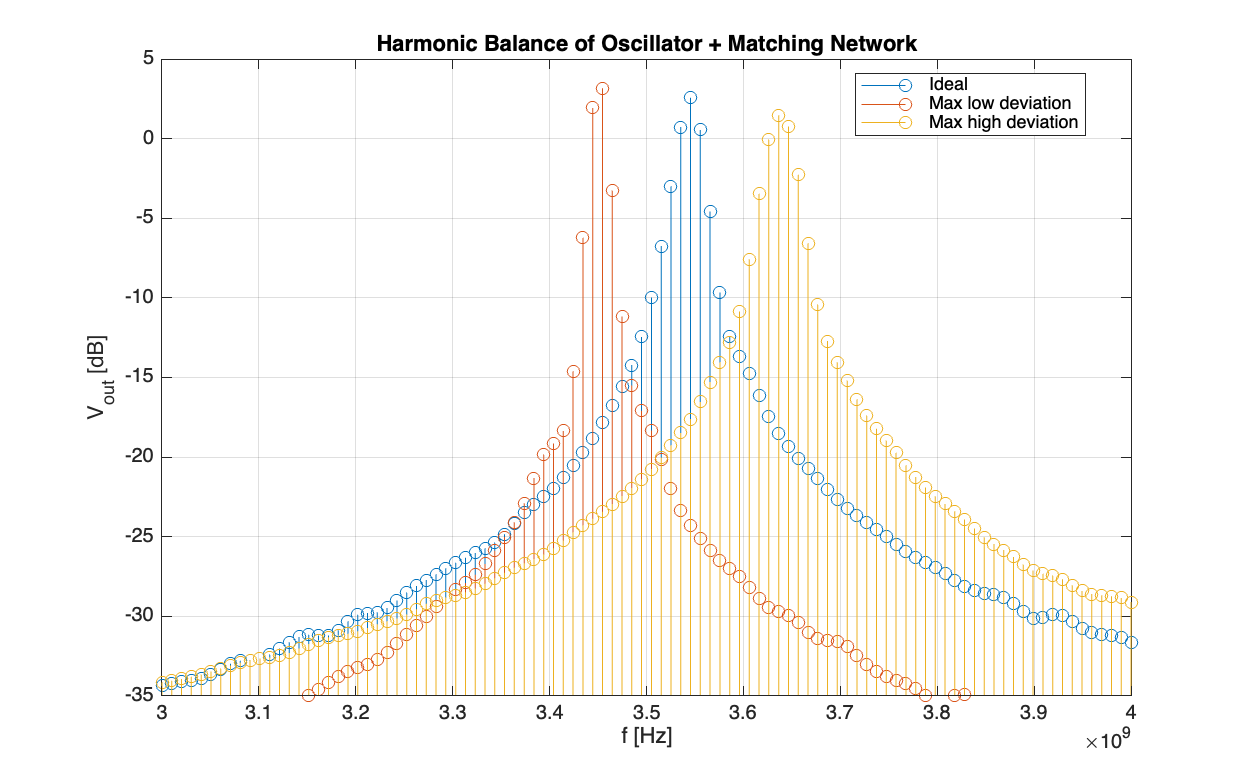
\includegraphics[width=\textwidth]{images/osc/VCO_spec_smoothed_with_peak_values.png}
        \caption{Spectral Analysis of Oscillator}
        \label{fig:osc_spec}
    \end{subfigure}
    \caption{Oscillator Outputs}
    \label{fig:osc}
\end{figure}
\end{comment}

\begin{figure}
    \centering
    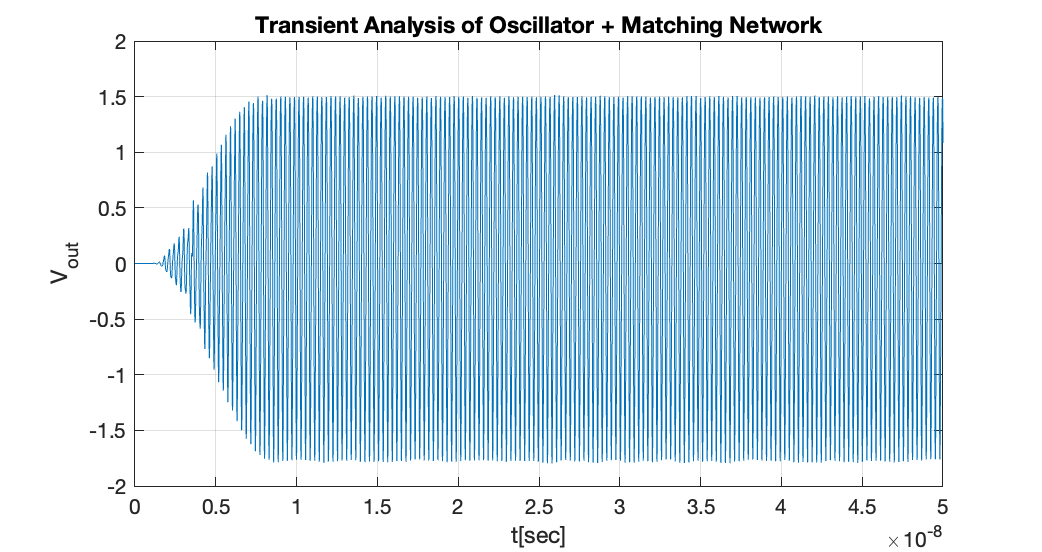
\includegraphics[width=0.95\textwidth]{images/osc/VCO_trans.png}
    \caption{Transient Analysis of Oscillator}
    \label{fig:osc_trans}
\end{figure}

Possible deviations due to non-idealities in the components need to be computed to ensure reliable functioning in the worst-case scenario. In accordance with manufacturer specification of the components used, the operating frequency was found to be in the range \(3.454[GHz]\to 3.636[GHz]\).\par

\begin{figure}
    \centering
    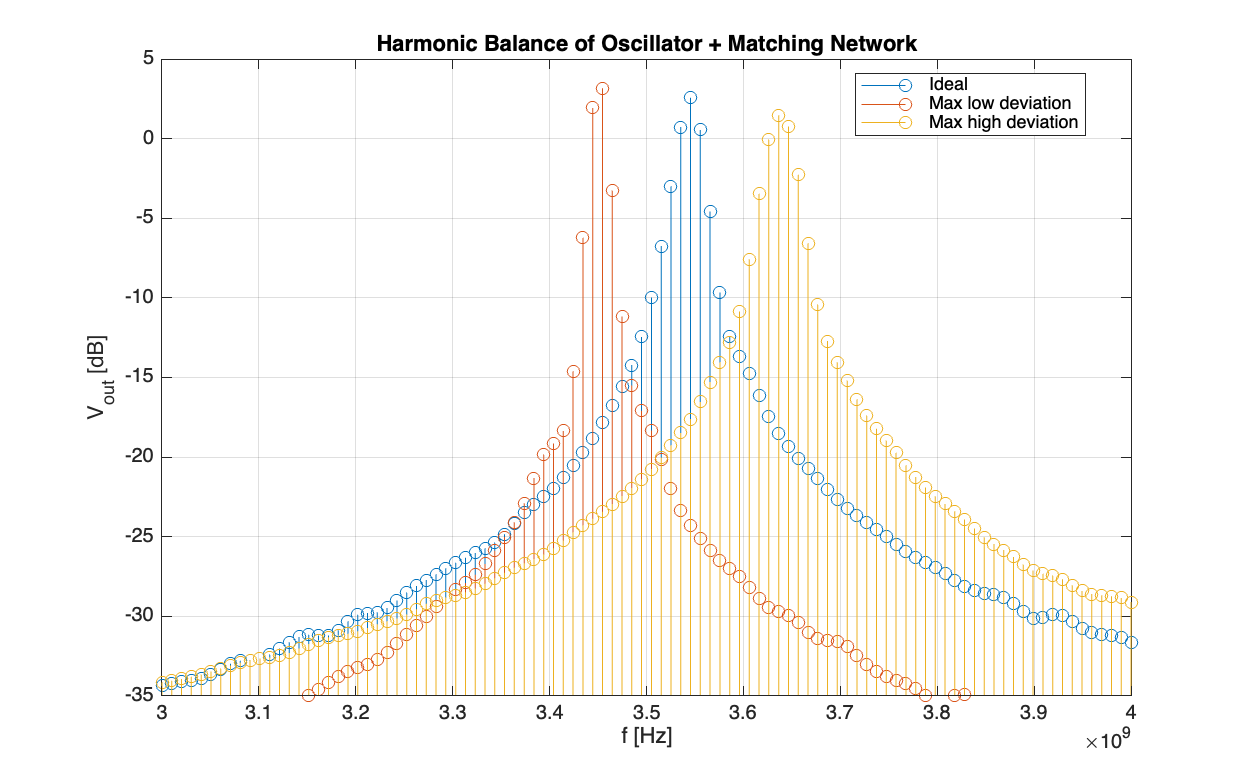
\includegraphics[width=0.9\textwidth]{images/osc/VCO_spec_smoothed_with_peak_values.png}
    \caption{Spectral Analysis of Oscillator}
    \label{fig:osc_spec}
\end{figure}

\begin{comment}
\begin{figure}
    \centering
    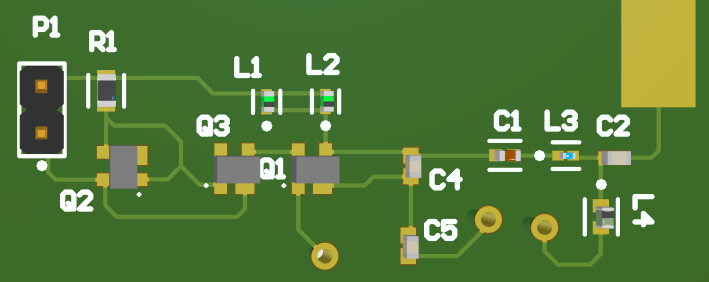
\includegraphics[width=0.85\textwidth]{images/layout/board3.png}
    \caption{3D Layout without Antenna}
    \label{fig:3DLayout}
\end{figure}
\end{comment}


\textbf{Antenna:}(\ref{fig:patch-antenna})
Scattering parameters were simulated for wide band micro-strip antenna as seen in Figure (\ref{fig:antenna_s}). The bandwidth was computed to be \(3.441[GHz]\to 3.642[Ghz]\), ensuring the deviations in oscillation frequency stay in \(S_{11}<-10[dB]\).

\begin{table}[H]
\centering
\caption{Far-Field Characteristics of Wideband Microstrip Antenna}
\label{table:antenna_characteristics}
\begin{tabularx}{0.7\linewidth}{|X|X|}
\hline
\textbf{Parameter} & \textbf{Value} \\
\hline
Main Lobe Magnitude & 6.22 dBi \\
Main Lobe Direction & 0.0 deg \\
Angular Width at 3 dB & 79.9 deg \\
Side Lobe Level & -15.6 dBi \\
\hline
\end{tabularx}
\end{table}